%\documentclass{standalone}
%\usepackage{tikz}
%\usetikzlibrary{patterns,plotmarks}
%\begin{document}
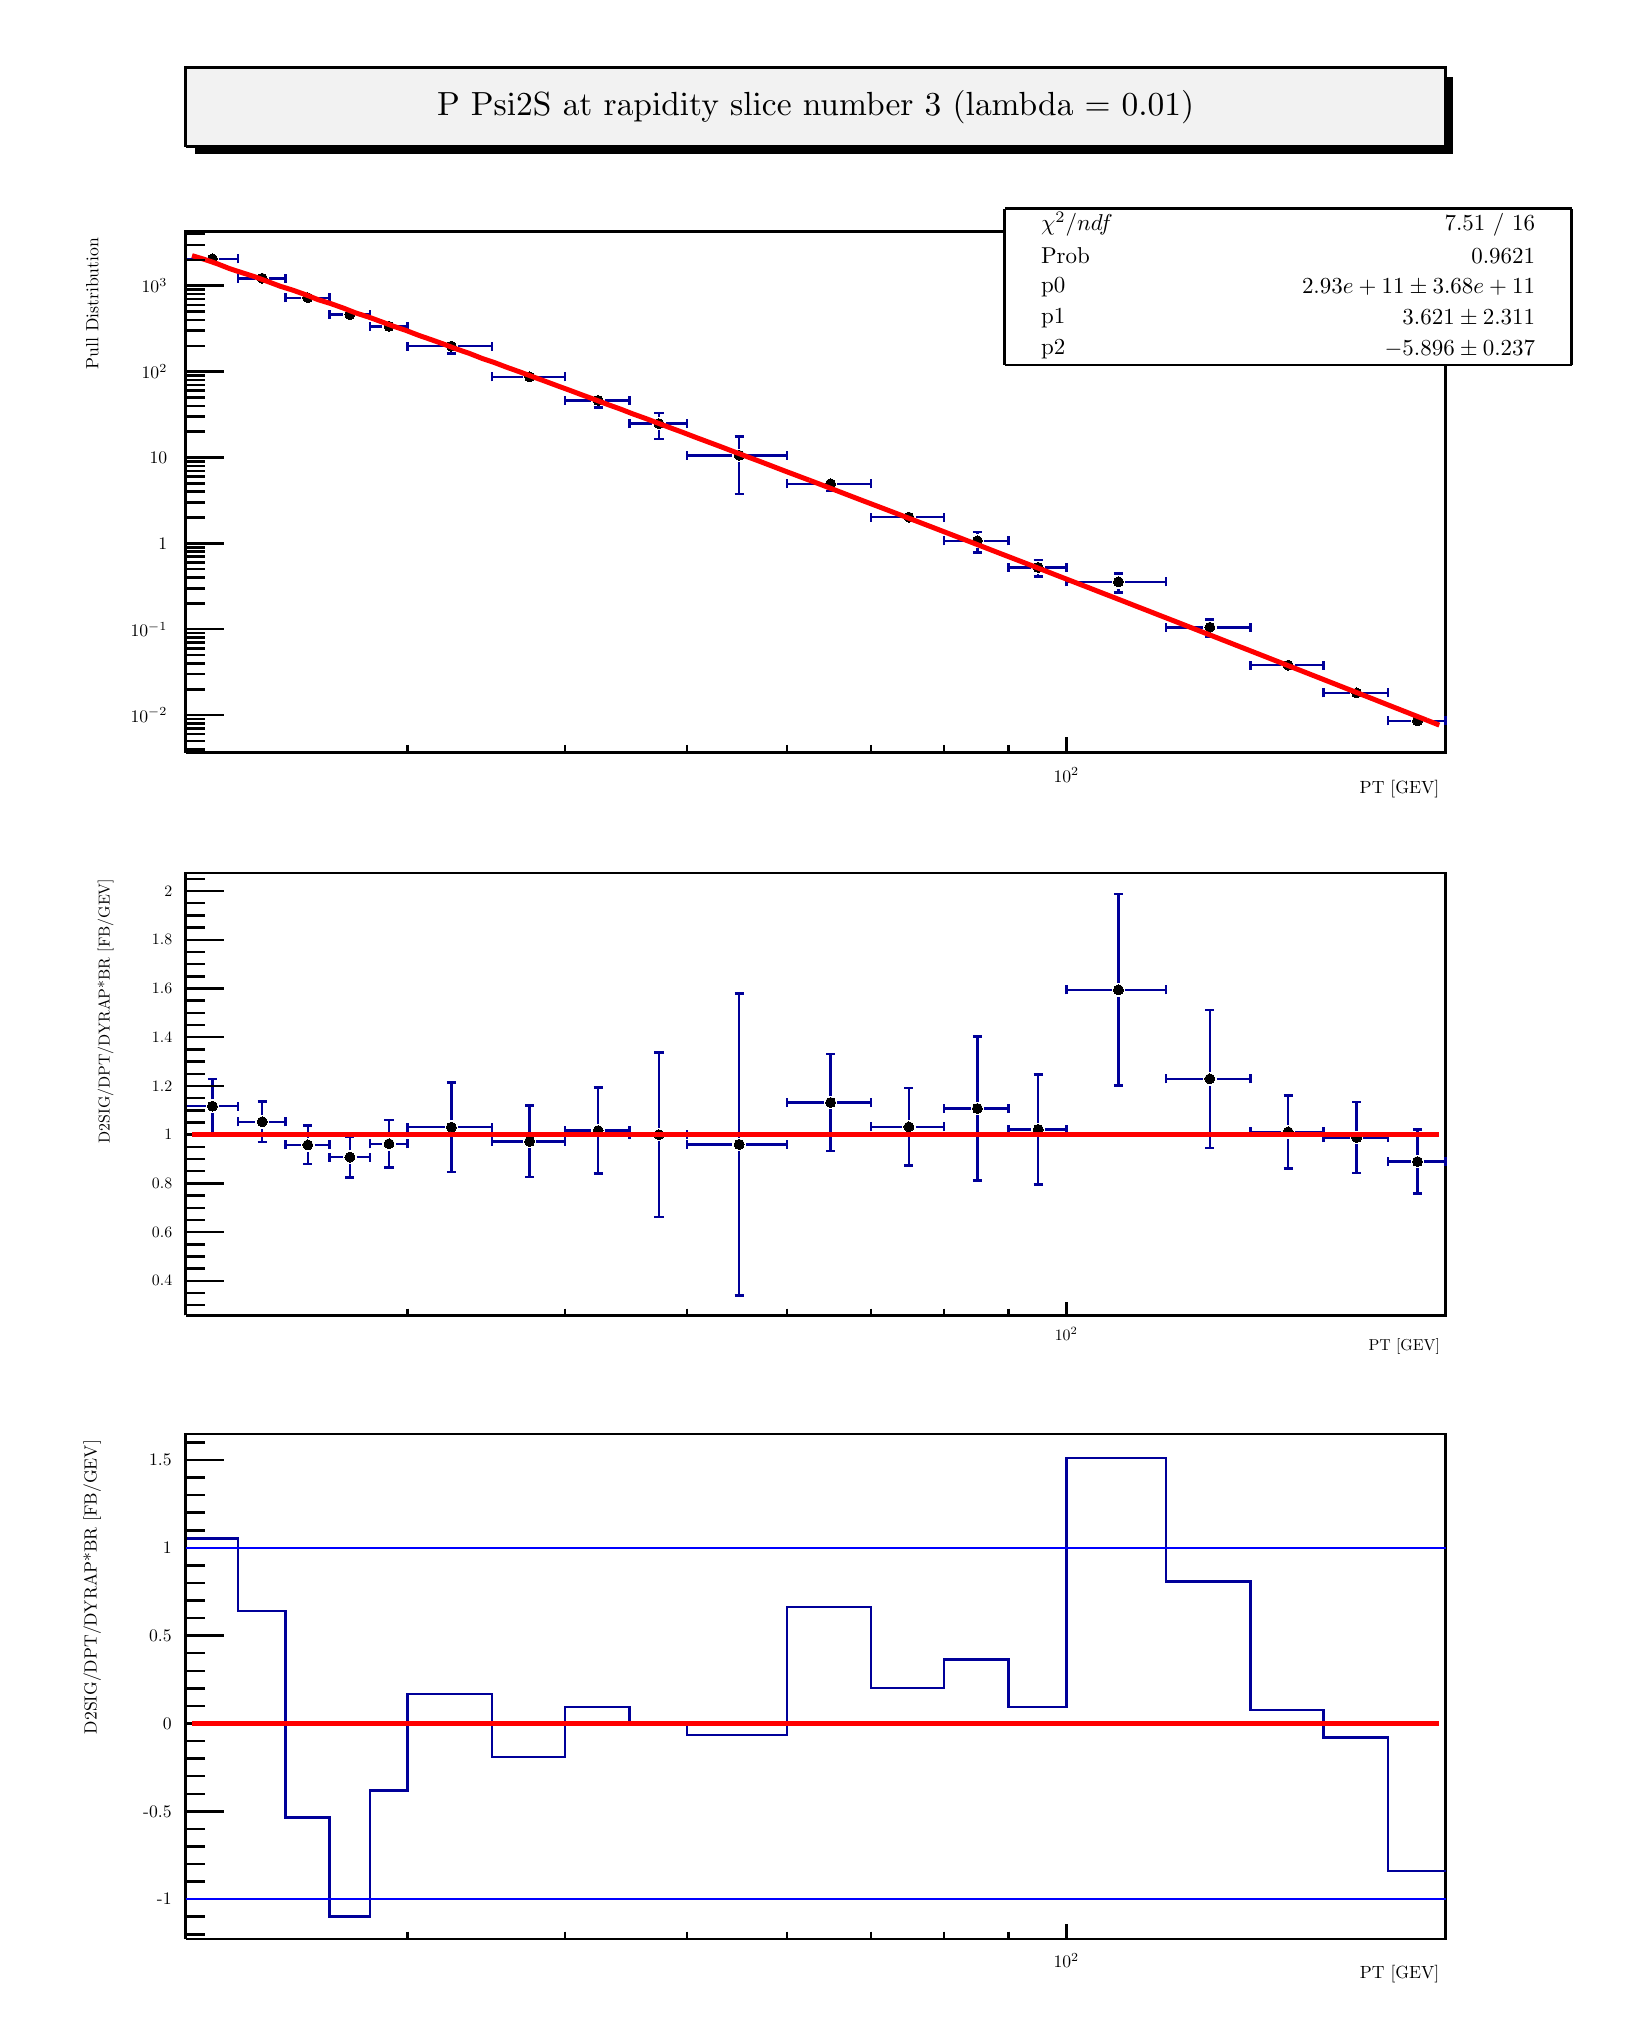
\begin{tikzpicture}
\def\CheckTikzLibraryLoaded#1{ \ifcsname tikz@library@#1@loaded\endcsname \else \PackageWarning{tikz}{usetikzlibrary{#1} is missing in the preamble.} \fi }
\CheckTikzLibraryLoaded{patterns}
\CheckTikzLibraryLoaded{plotmarks}
\pgfdeclareplotmark{cross} {
\pgfpathmoveto{\pgfpoint{-0.3\pgfplotmarksize}{\pgfplotmarksize}}
\pgfpathlineto{\pgfpoint{+0.3\pgfplotmarksize}{\pgfplotmarksize}}
\pgfpathlineto{\pgfpoint{+0.3\pgfplotmarksize}{0.3\pgfplotmarksize}}
\pgfpathlineto{\pgfpoint{+1\pgfplotmarksize}{0.3\pgfplotmarksize}}
\pgfpathlineto{\pgfpoint{+1\pgfplotmarksize}{-0.3\pgfplotmarksize}}
\pgfpathlineto{\pgfpoint{+0.3\pgfplotmarksize}{-0.3\pgfplotmarksize}}
\pgfpathlineto{\pgfpoint{+0.3\pgfplotmarksize}{-1.\pgfplotmarksize}}
\pgfpathlineto{\pgfpoint{-0.3\pgfplotmarksize}{-1.\pgfplotmarksize}}
\pgfpathlineto{\pgfpoint{-0.3\pgfplotmarksize}{-0.3\pgfplotmarksize}}
\pgfpathlineto{\pgfpoint{-1.\pgfplotmarksize}{-0.3\pgfplotmarksize}}
\pgfpathlineto{\pgfpoint{-1.\pgfplotmarksize}{0.3\pgfplotmarksize}}
\pgfpathlineto{\pgfpoint{-0.3\pgfplotmarksize}{0.3\pgfplotmarksize}}
\pgfpathclose
\pgfusepathqstroke
}
\pgfdeclareplotmark{cross*} {
\pgfpathmoveto{\pgfpoint{-0.3\pgfplotmarksize}{\pgfplotmarksize}}
\pgfpathlineto{\pgfpoint{+0.3\pgfplotmarksize}{\pgfplotmarksize}}
\pgfpathlineto{\pgfpoint{+0.3\pgfplotmarksize}{0.3\pgfplotmarksize}}
\pgfpathlineto{\pgfpoint{+1\pgfplotmarksize}{0.3\pgfplotmarksize}}
\pgfpathlineto{\pgfpoint{+1\pgfplotmarksize}{-0.3\pgfplotmarksize}}
\pgfpathlineto{\pgfpoint{+0.3\pgfplotmarksize}{-0.3\pgfplotmarksize}}
\pgfpathlineto{\pgfpoint{+0.3\pgfplotmarksize}{-1.\pgfplotmarksize}}
\pgfpathlineto{\pgfpoint{-0.3\pgfplotmarksize}{-1.\pgfplotmarksize}}
\pgfpathlineto{\pgfpoint{-0.3\pgfplotmarksize}{-0.3\pgfplotmarksize}}
\pgfpathlineto{\pgfpoint{-1.\pgfplotmarksize}{-0.3\pgfplotmarksize}}
\pgfpathlineto{\pgfpoint{-1.\pgfplotmarksize}{0.3\pgfplotmarksize}}
\pgfpathlineto{\pgfpoint{-0.3\pgfplotmarksize}{0.3\pgfplotmarksize}}
\pgfpathclose
\pgfusepathqfillstroke
}
\pgfdeclareplotmark{newstar} {
\pgfpathmoveto{\pgfqpoint{0pt}{\pgfplotmarksize}}
\pgfpathlineto{\pgfqpointpolar{44}{0.5\pgfplotmarksize}}
\pgfpathlineto{\pgfqpointpolar{18}{\pgfplotmarksize}}
\pgfpathlineto{\pgfqpointpolar{-20}{0.5\pgfplotmarksize}}
\pgfpathlineto{\pgfqpointpolar{-54}{\pgfplotmarksize}}
\pgfpathlineto{\pgfqpointpolar{-90}{0.5\pgfplotmarksize}}
\pgfpathlineto{\pgfqpointpolar{234}{\pgfplotmarksize}}
\pgfpathlineto{\pgfqpointpolar{198}{0.5\pgfplotmarksize}}
\pgfpathlineto{\pgfqpointpolar{162}{\pgfplotmarksize}}
\pgfpathlineto{\pgfqpointpolar{134}{0.5\pgfplotmarksize}}
\pgfpathclose
\pgfusepathqstroke
}
\pgfdeclareplotmark{newstar*} {
\pgfpathmoveto{\pgfqpoint{0pt}{\pgfplotmarksize}}
\pgfpathlineto{\pgfqpointpolar{44}{0.5\pgfplotmarksize}}
\pgfpathlineto{\pgfqpointpolar{18}{\pgfplotmarksize}}
\pgfpathlineto{\pgfqpointpolar{-20}{0.5\pgfplotmarksize}}
\pgfpathlineto{\pgfqpointpolar{-54}{\pgfplotmarksize}}
\pgfpathlineto{\pgfqpointpolar{-90}{0.5\pgfplotmarksize}}
\pgfpathlineto{\pgfqpointpolar{234}{\pgfplotmarksize}}
\pgfpathlineto{\pgfqpointpolar{198}{0.5\pgfplotmarksize}}
\pgfpathlineto{\pgfqpointpolar{162}{\pgfplotmarksize}}
\pgfpathlineto{\pgfqpointpolar{134}{0.5\pgfplotmarksize}}
\pgfpathclose
\pgfusepathqfillstroke
}
\definecolor{c}{rgb}{1,1,1};
\draw [color=c, fill=c] (0,0) rectangle (20,25.0716);
\definecolor{c}{rgb}{0.95,0.95,0.95};
\draw [color=c, fill=c] (2,23.5673) rectangle (18,24.5702);
\definecolor{c}{rgb}{0,0,0};
\draw [c, fill=c] (2.12894,23.5673) -- (2.12894,23.4814) -- (18.086,23.4814) -- (18.086,24.4413) -- (18,24.4413) -- (18,23.5673);
\draw [c,line width=0.9] (2,23.5673) -- (2,24.5702) -- (18,24.5702) -- (18,23.5673) -- (2,23.5673);
\draw (10,24.0688) node[scale=1.20912, color=c, rotate=0]{P Psi2S at rapidity slice number 3 (lambda = 0.01)};
\definecolor{c}{rgb}{1,1,1};
\draw [color=c, fill=c] (0,15.043) rectangle (20,23.3166);
\draw [color=c, fill=c] (2,15.8703) rectangle (18,22.4893);
\definecolor{c}{rgb}{0,0,0};
\draw [c,line width=0.9] (2,15.8703) -- (2,22.4893) -- (18,22.4893) -- (18,15.8703) -- (2,15.8703);
\definecolor{c}{rgb}{1,1,1};
\draw [color=c, fill=c] (2,15.8703) rectangle (18,22.4893);
\definecolor{c}{rgb}{0,0,0};
\draw [c,line width=0.9] (2,15.8703) -- (2,22.4893) -- (18,22.4893) -- (18,15.8703) -- (2,15.8703);
\definecolor{c}{rgb}{0,0,0.6};
\draw [c,line width=0.9] (2,22.1416) -- (2.25307,22.1416);
\draw [c,line width=0.9] (2.42499,22.1416) -- (2.66228,22.1416);
\draw [c,line width=0.9] (2,22.0843) -- (2,22.199);
\draw [c,line width=0.9] (2.66228,22.0843) -- (2.66228,22.199);
\definecolor{c}{rgb}{0,0,0};
\foreach \P in {(2.33903,22.1416)}{\draw[mark options={color=c,fill=c},mark size=1.801802pt, line width=0.000000pt, mark=*] plot coordinates {\P};}
\definecolor{c}{rgb}{0,0,0.6};
\draw [c,line width=0.9] (2.66228,21.8956) -- (2.88521,21.8956);
\draw [c,line width=0.9] (3.05713,21.8956) -- (3.2669,21.8956);
\draw [c,line width=0.9] (2.66228,21.8383) -- (2.66228,21.9529);
\draw [c,line width=0.9] (3.2669,21.8383) -- (3.2669,21.9529);
\definecolor{c}{rgb}{0,0,0};
\foreach \P in {(2.97117,21.8956)}{\draw[mark options={color=c,fill=c},mark size=1.801802pt, line width=0.000000pt, mark=*] plot coordinates {\P};}
\definecolor{c}{rgb}{0,0,0.6};
\draw [c,line width=0.9] (3.2669,21.6484) -- (3.4646,21.6484);
\draw [c,line width=0.9] (3.63652,21.6484) -- (3.82309,21.6484);
\draw [c,line width=0.9] (3.2669,21.5911) -- (3.2669,21.7057);
\draw [c,line width=0.9] (3.82309,21.5911) -- (3.82309,21.7057);
\definecolor{c}{rgb}{0,0,0};
\foreach \P in {(3.55056,21.6484)}{\draw[mark options={color=c,fill=c},mark size=1.801802pt, line width=0.000000pt, mark=*] plot coordinates {\P};}
\definecolor{c}{rgb}{0,0,0.6};
\draw [c,line width=0.9] (3.82309,21.4346) -- (3.99938,21.4346);
\draw [c,line width=0.9] (4.1713,21.4346) -- (4.33805,21.4346);
\draw [c,line width=0.9] (3.82309,21.3772) -- (3.82309,21.4919);
\draw [c,line width=0.9] (4.33805,21.3772) -- (4.33805,21.4919);
\definecolor{c}{rgb}{0,0,0};
\foreach \P in {(4.08534,21.4346)}{\draw[mark options={color=c,fill=c},mark size=1.801802pt, line width=0.000000pt, mark=*] plot coordinates {\P};}
\definecolor{c}{rgb}{0,0,0.6};
\draw [c,line width=0.9] (4.33805,21.2855) -- (4.49593,21.2855);
\draw [c,line width=0.9] (4.66785,21.2855) -- (4.81746,21.2855);
\draw [c,line width=0.9] (4.33805,21.2282) -- (4.33805,21.3428);
\draw [c,line width=0.9] (4.81746,21.2282) -- (4.81746,21.3428);
\definecolor{c}{rgb}{0,0,0};
\foreach \P in {(4.58189,21.2855)}{\draw[mark options={color=c,fill=c},mark size=1.801802pt, line width=0.000000pt, mark=*] plot coordinates {\P};}
\definecolor{c}{rgb}{0,0,0.6};
\draw [c,line width=0.9] (5.37365,20.9401) -- (5.37365,20.9473);
\draw [c,line width=0.9] (4.81746,21.0332) -- (5.28769,21.0332);
\draw [c,line width=0.9] (5.45961,21.0332) -- (5.88861,21.0332);
\draw [c,line width=0.9] (5.31635,20.9401) -- (5.43096,20.9401);
\draw [c,line width=0.9] (4.81746,20.9759) -- (4.81746,21.0905);
\draw [c,line width=0.9] (5.88861,20.9759) -- (5.88861,21.0905);
\definecolor{c}{rgb}{0,0,0};
\foreach \P in {(5.37365,21.0332)}{\draw[mark options={color=c,fill=c},mark size=1.801802pt, line width=0.000000pt, mark=*] plot coordinates {\P};}
\definecolor{c}{rgb}{0,0,0.6};
\draw [c,line width=0.9] (5.88861,20.6435) -- (6.28206,20.6435);
\draw [c,line width=0.9] (6.45398,20.6435) -- (6.81648,20.6435);
\draw [c,line width=0.9] (5.88861,20.5862) -- (5.88861,20.7008);
\draw [c,line width=0.9] (6.81648,20.5862) -- (6.81648,20.7008);
\definecolor{c}{rgb}{0,0,0};
\foreach \P in {(6.36802,20.6435)}{\draw[mark options={color=c,fill=c},mark size=1.801802pt, line width=0.000000pt, mark=*] plot coordinates {\P};}
\definecolor{c}{rgb}{0,0,0.6};
\draw [c,line width=0.9] (7.23774,20.2538) -- (7.23774,20.2582);
\draw [c,line width=0.9] (6.81648,20.3442) -- (7.15178,20.3442);
\draw [c,line width=0.9] (7.3237,20.3442) -- (7.63492,20.3442);
\draw [c,line width=0.9] (7.18044,20.2538) -- (7.29505,20.2538);
\draw [c,line width=0.9] (6.81648,20.2869) -- (6.81648,20.4015);
\draw [c,line width=0.9] (7.63492,20.2869) -- (7.63492,20.4015);
\definecolor{c}{rgb}{0,0,0};
\foreach \P in {(7.23774,20.3442)}{\draw[mark options={color=c,fill=c},mark size=1.801802pt, line width=0.000000pt, mark=*] plot coordinates {\P};}
\definecolor{c}{rgb}{0,0,0.6};
\draw [c,line width=0.9] (8.01062,19.8541) -- (8.01062,19.9629);
\draw [c,line width=0.9] (8.01062,20.1349) -- (8.01062,20.1866);
\draw [c,line width=0.9] (7.63492,20.0489) -- (7.92466,20.0489);
\draw [c,line width=0.9] (8.09658,20.0489) -- (8.36704,20.0489);
\draw [c,line width=0.9] (7.95331,19.8541) -- (8.06792,19.8541);
\draw [c,line width=0.9] (7.95331,20.1866) -- (8.06792,20.1866);
\draw [c,line width=0.9] (7.63492,19.9916) -- (7.63492,20.1062);
\draw [c,line width=0.9] (8.36704,19.9916) -- (8.36704,20.1062);
\definecolor{c}{rgb}{0,0,0};
\foreach \P in {(8.01062,20.0489)}{\draw[mark options={color=c,fill=c},mark size=1.801802pt, line width=0.000000pt, mark=*] plot coordinates {\P};}
\definecolor{c}{rgb}{0,0,0.6};
\draw [c,line width=0.9] (9.02932,19.1566) -- (9.02932,19.5615);
\draw [c,line width=0.9] (9.02932,19.7334) -- (9.02932,19.8833);
\draw [c,line width=0.9] (8.36704,19.6475) -- (8.94336,19.6475);
\draw [c,line width=0.9] (9.11528,19.6475) -- (9.63394,19.6475);
\draw [c,line width=0.9] (8.97202,19.1566) -- (9.08663,19.1566);
\draw [c,line width=0.9] (8.97202,19.8833) -- (9.08663,19.8833);
\draw [c,line width=0.9] (8.36704,19.5902) -- (8.36704,19.7048);
\draw [c,line width=0.9] (9.63394,19.5902) -- (9.63394,19.7048);
\definecolor{c}{rgb}{0,0,0};
\foreach \P in {(9.02932,19.6475)}{\draw[mark options={color=c,fill=c},mark size=1.801802pt, line width=0.000000pt, mark=*] plot coordinates {\P};}
\definecolor{c}{rgb}{0,0,0.6};
\draw [c,line width=0.9] (10.1901,19.1937) -- (10.1901,19.1996);
\draw [c,line width=0.9] (9.63394,19.2856) -- (10.1042,19.2856);
\draw [c,line width=0.9] (10.2761,19.2856) -- (10.7051,19.2856);
\draw [c,line width=0.9] (10.1328,19.1937) -- (10.2474,19.1937);
\draw [c,line width=0.9] (9.63394,19.2283) -- (9.63394,19.3429);
\draw [c,line width=0.9] (10.7051,19.2283) -- (10.7051,19.3429);
\definecolor{c}{rgb}{0,0,0};
\foreach \P in {(10.1901,19.2856)}{\draw[mark options={color=c,fill=c},mark size=1.801802pt, line width=0.000000pt, mark=*] plot coordinates {\P};}
\definecolor{c}{rgb}{0,0,0.6};
\draw [c,line width=0.9] (10.7051,18.8619) -- (11.0985,18.8619);
\draw [c,line width=0.9] (11.2705,18.8619) -- (11.633,18.8619);
\draw [c,line width=0.9] (10.7051,18.8046) -- (10.7051,18.9192);
\draw [c,line width=0.9] (11.633,18.8046) -- (11.633,18.9192);
\definecolor{c}{rgb}{0,0,0};
\foreach \P in {(11.1845,18.8619)}{\draw[mark options={color=c,fill=c},mark size=1.801802pt, line width=0.000000pt, mark=*] plot coordinates {\P};}
\definecolor{c}{rgb}{0,0,0.6};
\draw [c,line width=0.9] (12.0542,18.4136) -- (12.0542,18.4749);
\draw [c,line width=0.9] (12.0542,18.6468) -- (12.0542,18.673);
\draw [c,line width=0.9] (11.633,18.5609) -- (11.9683,18.5609);
\draw [c,line width=0.9] (12.1402,18.5609) -- (12.4514,18.5609);
\draw [c,line width=0.9] (11.9969,18.4136) -- (12.1115,18.4136);
\draw [c,line width=0.9] (11.9969,18.673) -- (12.1115,18.673);
\draw [c,line width=0.9] (11.633,18.5036) -- (11.633,18.6182);
\draw [c,line width=0.9] (12.4514,18.5036) -- (12.4514,18.6182);
\definecolor{c}{rgb}{0,0,0};
\foreach \P in {(12.0542,18.5609)}{\draw[mark options={color=c,fill=c},mark size=1.801802pt, line width=0.000000pt, mark=*] plot coordinates {\P};}
\definecolor{c}{rgb}{0,0,0.6};
\draw [c,line width=0.9] (12.8271,18.1054) -- (12.8271,18.1381);
\draw [c,line width=0.9] (12.8271,18.31) -- (12.8271,18.3189);
\draw [c,line width=0.9] (12.4514,18.224) -- (12.7411,18.224);
\draw [c,line width=0.9] (12.9131,18.224) -- (13.1835,18.224);
\draw [c,line width=0.9] (12.7698,18.1054) -- (12.8844,18.1054);
\draw [c,line width=0.9] (12.7698,18.3189) -- (12.8844,18.3189);
\draw [c,line width=0.9] (12.4514,18.1667) -- (12.4514,18.2814);
\draw [c,line width=0.9] (13.1835,18.1667) -- (13.1835,18.2814);
\definecolor{c}{rgb}{0,0,0};
\foreach \P in {(12.8271,18.224)}{\draw[mark options={color=c,fill=c},mark size=1.801802pt, line width=0.000000pt, mark=*] plot coordinates {\P};}
\definecolor{c}{rgb}{0,0,0.6};
\draw [c,line width=0.9] (13.8458,17.9054) -- (13.8458,17.9535);
\draw [c,line width=0.9] (13.8458,18.1255) -- (13.8458,18.1439);
\draw [c,line width=0.9] (13.1835,18.0395) -- (13.7598,18.0395);
\draw [c,line width=0.9] (13.9318,18.0395) -- (14.4504,18.0395);
\draw [c,line width=0.9] (13.7885,17.9054) -- (13.9031,17.9054);
\draw [c,line width=0.9] (13.7885,18.1439) -- (13.9031,18.1439);
\draw [c,line width=0.9] (13.1835,17.9822) -- (13.1835,18.0968);
\draw [c,line width=0.9] (14.4504,17.9822) -- (14.4504,18.0968);
\definecolor{c}{rgb}{0,0,0};
\foreach \P in {(13.8458,18.0395)}{\draw[mark options={color=c,fill=c},mark size=1.801802pt, line width=0.000000pt, mark=*] plot coordinates {\P};}
\definecolor{c}{rgb}{0,0,0.6};
\draw [c,line width=0.9] (15.0066,17.3395) -- (15.0066,17.3776);
\draw [c,line width=0.9] (15.0066,17.5495) -- (15.0066,17.5618);
\draw [c,line width=0.9] (14.4504,17.4636) -- (14.9207,17.4636);
\draw [c,line width=0.9] (15.0926,17.4636) -- (15.5216,17.4636);
\draw [c,line width=0.9] (14.9493,17.3395) -- (15.0639,17.3395);
\draw [c,line width=0.9] (14.9493,17.5618) -- (15.0639,17.5618);
\draw [c,line width=0.9] (14.4504,17.4063) -- (14.4504,17.5209);
\draw [c,line width=0.9] (15.5216,17.4063) -- (15.5216,17.5209);
\definecolor{c}{rgb}{0,0,0};
\foreach \P in {(15.0066,17.4636)}{\draw[mark options={color=c,fill=c},mark size=1.801802pt, line width=0.000000pt, mark=*] plot coordinates {\P};}
\definecolor{c}{rgb}{0,0,0.6};
\draw [c,line width=0.9] (15.5216,16.9817) -- (15.915,16.9817);
\draw [c,line width=0.9] (16.0869,16.9817) -- (16.4494,16.9817);
\draw [c,line width=0.9] (15.5216,16.9244) -- (15.5216,17.039);
\draw [c,line width=0.9] (16.4494,16.9244) -- (16.4494,17.039);
\definecolor{c}{rgb}{0,0,0};
\foreach \P in {(16.001,16.9817)}{\draw[mark options={color=c,fill=c},mark size=1.801802pt, line width=0.000000pt, mark=*] plot coordinates {\P};}
\definecolor{c}{rgb}{0,0,0.6};
\draw [c,line width=0.9] (16.4494,16.629) -- (16.7847,16.629);
\draw [c,line width=0.9] (16.9567,16.629) -- (17.2679,16.629);
\draw [c,line width=0.9] (16.4494,16.5717) -- (16.4494,16.6863);
\draw [c,line width=0.9] (17.2679,16.5717) -- (17.2679,16.6863);
\definecolor{c}{rgb}{0,0,0};
\foreach \P in {(16.8707,16.629)}{\draw[mark options={color=c,fill=c},mark size=1.801802pt, line width=0.000000pt, mark=*] plot coordinates {\P};}
\definecolor{c}{rgb}{0,0,0.6};
\draw [c,line width=0.9] (17.2679,16.2745) -- (17.5576,16.2745);
\draw [c,line width=0.9] (17.7295,16.2745) -- (18,16.2745);
\draw [c,line width=0.9] (17.2679,16.2172) -- (17.2679,16.3318);
\draw [c,line width=0.9] (18,16.2172) -- (18,16.3318);
\definecolor{c}{rgb}{0,0,0};
\foreach \P in {(17.6436,16.2745)}{\draw[mark options={color=c,fill=c},mark size=1.801802pt, line width=0.000000pt, mark=*] plot coordinates {\P};}
\definecolor{c}{rgb}{1,0,0};
\draw [c,line width=1.8] (2.08046,22.183) -- (2.24046,22.135) -- (2.40046,22.0802) -- (2.56046,22.0168) -- (2.72046,21.9651) -- (2.88046,21.9138) -- (3.04046,21.8549) -- (3.20046,21.7945) -- (3.36046,21.7447) -- (3.52046,21.6877) -- (3.68046,21.6244)
 -- (3.84046,21.5747) -- (4.00046,21.5178) -- (4.16046,21.455) -- (4.32046,21.404) -- (4.48046,21.3455) -- (4.64046,21.2856) -- (4.80046,21.2322) -- (4.96046,21.1705) -- (5.12046,21.1153) -- (5.28046,21.058) -- (5.44046,20.997) -- (5.60046,20.9424)
 -- (5.76046,20.8792) -- (5.92046,20.8254) -- (6.08046,20.7644) -- (6.24046,20.7077) -- (6.40046,20.6479) -- (6.56046,20.5898) -- (6.72046,20.5302) -- (6.88046,20.4718) -- (7.04046,20.4116) -- (7.20046,20.3536) -- (7.36046,20.2921) --
 (7.52046,20.2349) -- (7.68046,20.1726) -- (7.84046,20.1154) -- (8.00046,20.0548) -- (8.16046,19.9945) -- (8.32046,19.9358) -- (8.48046,19.8742) -- (8.64046,19.8148) -- (8.80046,19.7552) -- (8.96046,19.6937) -- (9.12046,19.6335) -- (9.28046,19.574)
 -- (9.44046,19.513) -- (9.60046,19.4512) -- (9.76046,19.3912) -- (9.92046,19.3311);
\draw [c,line width=1.8] (9.92046,19.3311) -- (10.0805,19.2702) -- (10.2405,19.2089) -- (10.4005,19.1473) -- (10.5605,19.0858) -- (10.7205,19.0252) -- (10.8805,18.9644) -- (11.0405,18.9032) -- (11.2005,18.842) -- (11.3605,18.7806) --
 (11.5205,18.7191) -- (11.6805,18.6575) -- (11.8405,18.5958) -- (12.0005,18.5341) -- (12.1605,18.4721) -- (12.3205,18.41) -- (12.4805,18.3484) -- (12.6405,18.2868) -- (12.8005,18.2251) -- (12.9605,18.163) -- (13.1205,18.1005) -- (13.2805,18.0387) --
 (13.4405,17.9768) -- (13.6005,17.9143) -- (13.7605,17.8523) -- (13.9205,17.7901) -- (14.0805,17.7274) -- (14.2405,17.6654) -- (14.4005,17.6027) -- (14.5605,17.5406) -- (14.7205,17.4779) -- (14.8805,17.4154) -- (15.0405,17.353) -- (15.2005,17.2902)
 -- (15.3605,17.2275) -- (15.5205,17.165) -- (15.6805,17.1024) -- (15.8405,17.0396) -- (16.0005,16.9767) -- (16.1605,16.9139) -- (16.3205,16.851) -- (16.4805,16.7882) -- (16.6405,16.7253) -- (16.8005,16.6624) -- (16.9605,16.5994) -- (17.1205,16.5364)
 -- (17.2805,16.4732) -- (17.4405,16.4103) -- (17.6005,16.3472) -- (17.7605,16.2841);
\draw [c,line width=1.8] (17.7605,16.2841) -- (17.9205,16.221);
\definecolor{c}{rgb}{1,1,1};
\draw [color=c, fill=c] (12.4,20.7932) rectangle (19.6,22.7788);
\definecolor{c}{rgb}{0,0,0};
\draw [c,line width=0.9] (12.4,20.7932) -- (19.6,20.7932);
\draw [c,line width=0.9] (19.6,20.7932) -- (19.6,22.7788);
\draw [c,line width=0.9] (19.6,22.7788) -- (12.4,22.7788);
\draw [c,line width=0.9] (12.4,22.7788) -- (12.4,20.7932);
\draw [anchor= west] (12.76,22.5803) node[scale=0.82945, color=c, rotate=0]{$\chi^{2} / ndf $};
\draw [anchor= east] (19.24,22.5803) node[scale=0.82945, color=c, rotate=0]{  7.51 / 16};
\draw [anchor= west] (12.76,22.1831) node[scale=0.82945, color=c, rotate=0]{Prob  };
\draw [anchor= east] (19.24,22.1831) node[scale=0.82945, color=c, rotate=0]{ 0.9621};
\draw [anchor= west] (12.76,21.786) node[scale=0.82945, color=c, rotate=0]{p0       };
\draw [anchor= east] (19.24,21.786) node[scale=0.82945, color=c, rotate=0]{$ 2.93e+11 \pm 3.68e+11$};
\draw [anchor= west] (12.76,21.3889) node[scale=0.82945, color=c, rotate=0]{p1       };
\draw [anchor= east] (19.24,21.3889) node[scale=0.82945, color=c, rotate=0]{$ 3.621 \pm 2.311$};
\draw [anchor= west] (12.76,20.9917) node[scale=0.82945, color=c, rotate=0]{p2       };
\draw [anchor= east] (19.24,20.9917) node[scale=0.82945, color=c, rotate=0]{$ -5.896 \pm 0.237$};
\draw [c,line width=0.9] (2,15.8703) -- (18,15.8703);
\draw [c,line width=0.9] (4.81745,15.9696) -- (4.81745,15.8703);
\draw [c,line width=0.9] (6.81647,15.9696) -- (6.81647,15.8703);
\draw [c,line width=0.9] (8.36703,15.9696) -- (8.36703,15.8703);
\draw [c,line width=0.9] (9.63393,15.9696) -- (9.63393,15.8703);
\draw [c,line width=0.9] (10.7051,15.9696) -- (10.7051,15.8703);
\draw [c,line width=0.9] (11.633,15.9696) -- (11.633,15.8703);
\draw [c,line width=0.9] (12.4514,15.9696) -- (12.4514,15.8703);
\draw [c,line width=0.9] (13.1835,16.0689) -- (13.1835,15.8703);
\draw [anchor=base] (13.1835,15.496) node[scale=0.638038, color=c, rotate=0]{$10^{2}$};
\draw [c,line width=0.9] (18,15.9696) -- (18,15.8703);
\draw [anchor= east] (18,15.407) node[scale=0.638038, color=c, rotate=0]{PT [GEV]};
\draw [c,line width=0.9] (2,15.8703) -- (2,22.4893);
\draw [c,line width=0.9] (2.24,15.9139) -- (2,15.9139);
\draw [c,line width=0.9] (2.24,16.0196) -- (2,16.0196);
\draw [c,line width=0.9] (2.24,16.1059) -- (2,16.1059);
\draw [c,line width=0.9] (2.24,16.1789) -- (2,16.1789);
\draw [c,line width=0.9] (2.24,16.2422) -- (2,16.2422);
\draw [c,line width=0.9] (2.24,16.298) -- (2,16.298);
\draw [c,line width=0.9] (2.48,16.3479) -- (2,16.3479);
\draw [anchor= east] (1.844,16.3479) node[scale=0.638038, color=c, rotate=0]{$10^{-2}$};
\draw [c,line width=0.9] (2.24,16.6762) -- (2,16.6762);
\draw [c,line width=0.9] (2.24,16.8683) -- (2,16.8683);
\draw [c,line width=0.9] (2.24,17.0045) -- (2,17.0045);
\draw [c,line width=0.9] (2.24,17.1102) -- (2,17.1102);
\draw [c,line width=0.9] (2.24,17.1966) -- (2,17.1966);
\draw [c,line width=0.9] (2.24,17.2696) -- (2,17.2696);
\draw [c,line width=0.9] (2.24,17.3328) -- (2,17.3328);
\draw [c,line width=0.9] (2.24,17.3886) -- (2,17.3886);
\draw [c,line width=0.9] (2.48,17.4385) -- (2,17.4385);
\draw [anchor= east] (1.844,17.4385) node[scale=0.638038, color=c, rotate=0]{$10^{-1}$};
\draw [c,line width=0.9] (2.24,17.7669) -- (2,17.7669);
\draw [c,line width=0.9] (2.24,17.9589) -- (2,17.9589);
\draw [c,line width=0.9] (2.24,18.0952) -- (2,18.0952);
\draw [c,line width=0.9] (2.24,18.2009) -- (2,18.2009);
\draw [c,line width=0.9] (2.24,18.2872) -- (2,18.2872);
\draw [c,line width=0.9] (2.24,18.3603) -- (2,18.3603);
\draw [c,line width=0.9] (2.24,18.4235) -- (2,18.4235);
\draw [c,line width=0.9] (2.24,18.4793) -- (2,18.4793);
\draw [c,line width=0.9] (2.48,18.5292) -- (2,18.5292);
\draw [anchor= east] (1.844,18.5292) node[scale=0.638038, color=c, rotate=0]{1};
\draw [c,line width=0.9] (2.24,18.8575) -- (2,18.8575);
\draw [c,line width=0.9] (2.24,19.0496) -- (2,19.0496);
\draw [c,line width=0.9] (2.24,19.1858) -- (2,19.1858);
\draw [c,line width=0.9] (2.24,19.2915) -- (2,19.2915);
\draw [c,line width=0.9] (2.24,19.3779) -- (2,19.3779);
\draw [c,line width=0.9] (2.24,19.4509) -- (2,19.4509);
\draw [c,line width=0.9] (2.24,19.5142) -- (2,19.5142);
\draw [c,line width=0.9] (2.24,19.5699) -- (2,19.5699);
\draw [c,line width=0.9] (2.48,19.6198) -- (2,19.6198);
\draw [anchor= east] (1.844,19.6198) node[scale=0.638038, color=c, rotate=0]{10};
\draw [c,line width=0.9] (2.24,19.9482) -- (2,19.9482);
\draw [c,line width=0.9] (2.24,20.1402) -- (2,20.1402);
\draw [c,line width=0.9] (2.24,20.2765) -- (2,20.2765);
\draw [c,line width=0.9] (2.24,20.3822) -- (2,20.3822);
\draw [c,line width=0.9] (2.24,20.4685) -- (2,20.4685);
\draw [c,line width=0.9] (2.24,20.5416) -- (2,20.5416);
\draw [c,line width=0.9] (2.24,20.6048) -- (2,20.6048);
\draw [c,line width=0.9] (2.24,20.6606) -- (2,20.6606);
\draw [c,line width=0.9] (2.48,20.7105) -- (2,20.7105);
\draw [anchor= east] (1.844,20.7105) node[scale=0.638038, color=c, rotate=0]{$10^{2}$};
\draw [c,line width=0.9] (2.24,21.0388) -- (2,21.0388);
\draw [c,line width=0.9] (2.24,21.2309) -- (2,21.2309);
\draw [c,line width=0.9] (2.24,21.3671) -- (2,21.3671);
\draw [c,line width=0.9] (2.24,21.4728) -- (2,21.4728);
\draw [c,line width=0.9] (2.24,21.5592) -- (2,21.5592);
\draw [c,line width=0.9] (2.24,21.6322) -- (2,21.6322);
\draw [c,line width=0.9] (2.24,21.6955) -- (2,21.6955);
\draw [c,line width=0.9] (2.24,21.7512) -- (2,21.7512);
\draw [c,line width=0.9] (2.48,21.8011) -- (2,21.8011);
\draw [anchor= east] (1.844,21.8011) node[scale=0.638038, color=c, rotate=0]{$10^{3}$};
\draw [c,line width=0.9] (2.24,22.1295) -- (2,22.1295);
\draw [c,line width=0.9] (2.24,22.3215) -- (2,22.3215);
\draw [c,line width=0.9] (2.24,22.4578) -- (2,22.4578);
\draw [anchor= east] (0.812894,22.4893) node[scale=0.638038, color=c, rotate=90]{Pull Distribution};
\definecolor{c}{rgb}{1,1,1};
\draw [color=c, fill=c] (12.4,20.7932) rectangle (19.6,22.7788);
\definecolor{c}{rgb}{0,0,0};
\draw [c,line width=0.9] (12.4,20.7932) -- (19.6,20.7932);
\draw [c,line width=0.9] (19.6,20.7932) -- (19.6,22.7788);
\draw [c,line width=0.9] (19.6,22.7788) -- (12.4,22.7788);
\draw [c,line width=0.9] (12.4,22.7788) -- (12.4,20.7932);
\draw [anchor= west] (12.76,22.5803) node[scale=0.82945, color=c, rotate=0]{$\chi^{2} / ndf $};
\draw [anchor= east] (19.24,22.5803) node[scale=0.82945, color=c, rotate=0]{  7.51 / 16};
\draw [anchor= west] (12.76,22.1831) node[scale=0.82945, color=c, rotate=0]{Prob  };
\draw [anchor= east] (19.24,22.1831) node[scale=0.82945, color=c, rotate=0]{ 0.9621};
\draw [anchor= west] (12.76,21.786) node[scale=0.82945, color=c, rotate=0]{p0       };
\draw [anchor= east] (19.24,21.786) node[scale=0.82945, color=c, rotate=0]{$ 2.93e+11 \pm 3.68e+11$};
\draw [anchor= west] (12.76,21.3889) node[scale=0.82945, color=c, rotate=0]{p1       };
\draw [anchor= east] (19.24,21.3889) node[scale=0.82945, color=c, rotate=0]{$ 3.621 \pm 2.311$};
\draw [anchor= west] (12.76,20.9917) node[scale=0.82945, color=c, rotate=0]{p2       };
\draw [anchor= east] (19.24,20.9917) node[scale=0.82945, color=c, rotate=0]{$ -5.896 \pm 0.237$};
\definecolor{c}{rgb}{1,1,1};
\draw [color=c, fill=c] (0,8.02292) rectangle (20,15.043);
\draw [color=c, fill=c] (2,8.72493) rectangle (18,14.341);
\definecolor{c}{rgb}{0,0,0};
\draw [c,line width=0.9] (2,8.72493) -- (2,14.341) -- (18,14.341) -- (18,8.72493) -- (2,8.72493);
\definecolor{c}{rgb}{1,1,1};
\draw [color=c, fill=c] (2,8.72493) rectangle (18,14.341);
\definecolor{c}{rgb}{0,0,0};
\draw [c,line width=0.9] (2,8.72493) -- (2,14.341) -- (18,14.341) -- (18,8.72493) -- (2,8.72493);
\definecolor{c}{rgb}{0,0,0.6};
\draw [c,line width=0.9] (2.33903,11.0379) -- (2.33903,11.2955);
\draw [c,line width=0.9] (2.33903,11.4674) -- (2.33903,11.7251);
\draw [c,line width=0.9] (2,11.3815) -- (2.25307,11.3815);
\draw [c,line width=0.9] (2.42499,11.3815) -- (2.66228,11.3815);
\draw [c,line width=0.9] (2.28172,11.0379) -- (2.39634,11.0379);
\draw [c,line width=0.9] (2.28172,11.7251) -- (2.39634,11.7251);
\draw [c,line width=0.9] (2,11.3242) -- (2,11.4388);
\draw [c,line width=0.9] (2.66228,11.3242) -- (2.66228,11.4388);
\definecolor{c}{rgb}{0,0,0};
\foreach \P in {(2.33903,11.3815)}{\draw[mark options={color=c,fill=c},mark size=1.801802pt, line width=0.000000pt, mark=*] plot coordinates {\P};}
\definecolor{c}{rgb}{0,0,0.6};
\draw [c,line width=0.9] (2.97117,10.9271) -- (2.97117,11.0975);
\draw [c,line width=0.9] (2.97117,11.2694) -- (2.97117,11.4398);
\draw [c,line width=0.9] (2.66228,11.1834) -- (2.88521,11.1834);
\draw [c,line width=0.9] (3.05713,11.1834) -- (3.2669,11.1834);
\draw [c,line width=0.9] (2.91386,10.9271) -- (3.02847,10.9271);
\draw [c,line width=0.9] (2.91386,11.4398) -- (3.02847,11.4398);
\draw [c,line width=0.9] (2.66228,11.1261) -- (2.66228,11.2407);
\draw [c,line width=0.9] (3.2669,11.1261) -- (3.2669,11.2407);
\definecolor{c}{rgb}{0,0,0};
\foreach \P in {(2.97117,11.1834)}{\draw[mark options={color=c,fill=c},mark size=1.801802pt, line width=0.000000pt, mark=*] plot coordinates {\P};}
\definecolor{c}{rgb}{0,0,0.6};
\draw [c,line width=0.9] (3.55056,10.6443) -- (3.55056,10.8029);
\draw [c,line width=0.9] (3.55056,10.9748) -- (3.55056,11.1334);
\draw [c,line width=0.9] (3.2669,10.8889) -- (3.4646,10.8889);
\draw [c,line width=0.9] (3.63652,10.8889) -- (3.82309,10.8889);
\draw [c,line width=0.9] (3.49325,10.6443) -- (3.60787,10.6443);
\draw [c,line width=0.9] (3.49325,11.1334) -- (3.60787,11.1334);
\draw [c,line width=0.9] (3.2669,10.8316) -- (3.2669,10.9462);
\draw [c,line width=0.9] (3.82309,10.8316) -- (3.82309,10.9462);
\definecolor{c}{rgb}{0,0,0};
\foreach \P in {(3.55056,10.8889)}{\draw[mark options={color=c,fill=c},mark size=1.801802pt, line width=0.000000pt, mark=*] plot coordinates {\P};}
\definecolor{c}{rgb}{0,0,0.6};
\draw [c,line width=0.9] (4.08534,10.4762) -- (4.08534,10.6493);
\draw [c,line width=0.9] (4.08534,10.8212) -- (4.08534,10.9943);
\draw [c,line width=0.9] (3.82309,10.7353) -- (3.99938,10.7353);
\draw [c,line width=0.9] (4.1713,10.7353) -- (4.33805,10.7353);
\draw [c,line width=0.9] (4.02803,10.4762) -- (4.14265,10.4762);
\draw [c,line width=0.9] (4.02803,10.9943) -- (4.14265,10.9943);
\draw [c,line width=0.9] (3.82309,10.678) -- (3.82309,10.7926);
\draw [c,line width=0.9] (4.33805,10.678) -- (4.33805,10.7926);
\definecolor{c}{rgb}{0,0,0};
\foreach \P in {(4.08534,10.7353)}{\draw[mark options={color=c,fill=c},mark size=1.801802pt, line width=0.000000pt, mark=*] plot coordinates {\P};}
\definecolor{c}{rgb}{0,0,0.6};
\draw [c,line width=0.9] (4.58189,10.6014) -- (4.58189,10.8183);
\draw [c,line width=0.9] (4.58189,10.9902) -- (4.58189,11.207);
\draw [c,line width=0.9] (4.33805,10.9042) -- (4.49593,10.9042);
\draw [c,line width=0.9] (4.66785,10.9042) -- (4.81746,10.9042);
\draw [c,line width=0.9] (4.52458,10.6014) -- (4.63919,10.6014);
\draw [c,line width=0.9] (4.52458,11.207) -- (4.63919,11.207);
\draw [c,line width=0.9] (4.33805,10.8469) -- (4.33805,10.9615);
\draw [c,line width=0.9] (4.81746,10.8469) -- (4.81746,10.9615);
\definecolor{c}{rgb}{0,0,0};
\foreach \P in {(4.58189,10.9042)}{\draw[mark options={color=c,fill=c},mark size=1.801802pt, line width=0.000000pt, mark=*] plot coordinates {\P};}
\definecolor{c}{rgb}{0,0,0.6};
\draw [c,line width=0.9] (5.37365,10.5454) -- (5.37365,11.0287);
\draw [c,line width=0.9] (5.37365,11.2006) -- (5.37365,11.6838);
\draw [c,line width=0.9] (4.81746,11.1146) -- (5.28769,11.1146);
\draw [c,line width=0.9] (5.45961,11.1146) -- (5.88861,11.1146);
\draw [c,line width=0.9] (5.31635,10.5454) -- (5.43096,10.5454);
\draw [c,line width=0.9] (5.31635,11.6838) -- (5.43096,11.6838);
\draw [c,line width=0.9] (4.81746,11.0573) -- (4.81746,11.1719);
\draw [c,line width=0.9] (5.88861,11.0573) -- (5.88861,11.1719);
\definecolor{c}{rgb}{0,0,0};
\foreach \P in {(5.37365,11.1146)}{\draw[mark options={color=c,fill=c},mark size=1.801802pt, line width=0.000000pt, mark=*] plot coordinates {\P};}
\definecolor{c}{rgb}{0,0,0.6};
\draw [c,line width=0.9] (6.36802,10.4798) -- (6.36802,10.8476);
\draw [c,line width=0.9] (6.36802,11.0195) -- (6.36802,11.3873);
\draw [c,line width=0.9] (5.88861,10.9336) -- (6.28206,10.9336);
\draw [c,line width=0.9] (6.45398,10.9336) -- (6.81648,10.9336);
\draw [c,line width=0.9] (6.31071,10.4798) -- (6.42533,10.4798);
\draw [c,line width=0.9] (6.31071,11.3873) -- (6.42533,11.3873);
\draw [c,line width=0.9] (5.88861,10.8763) -- (5.88861,10.9909);
\draw [c,line width=0.9] (6.81648,10.8763) -- (6.81648,10.9909);
\definecolor{c}{rgb}{0,0,0};
\foreach \P in {(6.36802,10.9336)}{\draw[mark options={color=c,fill=c},mark size=1.801802pt, line width=0.000000pt, mark=*] plot coordinates {\P};}
\definecolor{c}{rgb}{0,0,0.6};
\draw [c,line width=0.9] (7.23774,10.5245) -- (7.23774,10.9849);
\draw [c,line width=0.9] (7.23774,11.1568) -- (7.23774,11.6173);
\draw [c,line width=0.9] (6.81648,11.0709) -- (7.15178,11.0709);
\draw [c,line width=0.9] (7.3237,11.0709) -- (7.63492,11.0709);
\draw [c,line width=0.9] (7.18044,10.5245) -- (7.29505,10.5245);
\draw [c,line width=0.9] (7.18044,11.6173) -- (7.29505,11.6173);
\draw [c,line width=0.9] (6.81648,11.0136) -- (6.81648,11.1282);
\draw [c,line width=0.9] (7.63492,11.0136) -- (7.63492,11.1282);
\definecolor{c}{rgb}{0,0,0};
\foreach \P in {(7.23774,11.0709)}{\draw[mark options={color=c,fill=c},mark size=1.801802pt, line width=0.000000pt, mark=*] plot coordinates {\P};}
\definecolor{c}{rgb}{0,0,0.6};
\draw [c,line width=0.9] (8.01062,9.97589) -- (8.01062,10.9332);
\draw [c,line width=0.9] (8.01062,11.1051) -- (8.01062,12.0624);
\draw [c,line width=0.9] (7.63492,11.0191) -- (7.92466,11.0191);
\draw [c,line width=0.9] (8.09658,11.0191) -- (8.36704,11.0191);
\draw [c,line width=0.9] (7.95331,9.97589) -- (8.06792,9.97589);
\draw [c,line width=0.9] (7.95331,12.0624) -- (8.06792,12.0624);
\draw [c,line width=0.9] (7.63492,10.9618) -- (7.63492,11.0764);
\draw [c,line width=0.9] (8.36704,10.9618) -- (8.36704,11.0764);
\definecolor{c}{rgb}{0,0,0};
\foreach \P in {(8.01062,11.0191)}{\draw[mark options={color=c,fill=c},mark size=1.801802pt, line width=0.000000pt, mark=*] plot coordinates {\P};}
\definecolor{c}{rgb}{0,0,0.6};
\draw [c,line width=0.9] (9.02932,8.97962) -- (9.02932,10.8106);
\draw [c,line width=0.9] (9.02932,10.9825) -- (9.02932,12.8135);
\draw [c,line width=0.9] (8.36704,10.8966) -- (8.94336,10.8966);
\draw [c,line width=0.9] (9.11528,10.8966) -- (9.63394,10.8966);
\draw [c,line width=0.9] (8.97202,8.97962) -- (9.08663,8.97962);
\draw [c,line width=0.9] (8.97202,12.8135) -- (9.08663,12.8135);
\draw [c,line width=0.9] (8.36704,10.8392) -- (8.36704,10.9539);
\draw [c,line width=0.9] (9.63394,10.8392) -- (9.63394,10.9539);
\definecolor{c}{rgb}{0,0,0};
\foreach \P in {(9.02932,10.8966)}{\draw[mark options={color=c,fill=c},mark size=1.801802pt, line width=0.000000pt, mark=*] plot coordinates {\P};}
\definecolor{c}{rgb}{0,0,0.6};
\draw [c,line width=0.9] (10.1901,10.8108) -- (10.1901,11.3421);
\draw [c,line width=0.9] (10.1901,11.5141) -- (10.1901,12.0454);
\draw [c,line width=0.9] (9.63394,11.4281) -- (10.1042,11.4281);
\draw [c,line width=0.9] (10.2761,11.4281) -- (10.7051,11.4281);
\draw [c,line width=0.9] (10.1328,10.8108) -- (10.2474,10.8108);
\draw [c,line width=0.9] (10.1328,12.0454) -- (10.2474,12.0454);
\draw [c,line width=0.9] (9.63394,11.3708) -- (9.63394,11.4854);
\draw [c,line width=0.9] (10.7051,11.3708) -- (10.7051,11.4854);
\definecolor{c}{rgb}{0,0,0};
\foreach \P in {(10.1901,11.4281)}{\draw[mark options={color=c,fill=c},mark size=1.801802pt, line width=0.000000pt, mark=*] plot coordinates {\P};}
\definecolor{c}{rgb}{0,0,0.6};
\draw [c,line width=0.9] (11.1845,10.6271) -- (11.1845,11.033);
\draw [c,line width=0.9] (11.1845,11.205) -- (11.1845,11.6109);
\draw [c,line width=0.9] (10.7051,11.119) -- (11.0985,11.119);
\draw [c,line width=0.9] (11.2705,11.119) -- (11.633,11.119);
\draw [c,line width=0.9] (11.1272,10.6271) -- (11.2418,10.6271);
\draw [c,line width=0.9] (11.1272,11.6109) -- (11.2418,11.6109);
\draw [c,line width=0.9] (10.7051,11.0617) -- (10.7051,11.1763);
\draw [c,line width=0.9] (11.633,11.0617) -- (11.633,11.1763);
\definecolor{c}{rgb}{0,0,0};
\foreach \P in {(11.1845,11.119)}{\draw[mark options={color=c,fill=c},mark size=1.801802pt, line width=0.000000pt, mark=*] plot coordinates {\P};}
\definecolor{c}{rgb}{0,0,0.6};
\draw [c,line width=0.9] (12.0542,10.4364) -- (12.0542,11.2658);
\draw [c,line width=0.9] (12.0542,11.4377) -- (12.0542,12.2671);
\draw [c,line width=0.9] (11.633,11.3518) -- (11.9683,11.3518);
\draw [c,line width=0.9] (12.1402,11.3518) -- (12.4514,11.3518);
\draw [c,line width=0.9] (11.9969,10.4364) -- (12.1115,10.4364);
\draw [c,line width=0.9] (11.9969,12.2671) -- (12.1115,12.2671);
\draw [c,line width=0.9] (11.633,11.2945) -- (11.633,11.4091);
\draw [c,line width=0.9] (12.4514,11.2945) -- (12.4514,11.4091);
\definecolor{c}{rgb}{0,0,0};
\foreach \P in {(12.0542,11.3518)}{\draw[mark options={color=c,fill=c},mark size=1.801802pt, line width=0.000000pt, mark=*] plot coordinates {\P};}
\definecolor{c}{rgb}{0,0,0.6};
\draw [c,line width=0.9] (12.8271,10.3856) -- (12.8271,11);
\draw [c,line width=0.9] (12.8271,11.1719) -- (12.8271,11.7862);
\draw [c,line width=0.9] (12.4514,11.0859) -- (12.7411,11.0859);
\draw [c,line width=0.9] (12.9131,11.0859) -- (13.1835,11.0859);
\draw [c,line width=0.9] (12.7698,10.3856) -- (12.8844,10.3856);
\draw [c,line width=0.9] (12.7698,11.7862) -- (12.8844,11.7862);
\draw [c,line width=0.9] (12.4514,11.0286) -- (12.4514,11.1432);
\draw [c,line width=0.9] (13.1835,11.0286) -- (13.1835,11.1432);
\definecolor{c}{rgb}{0,0,0};
\foreach \P in {(12.8271,11.0859)}{\draw[mark options={color=c,fill=c},mark size=1.801802pt, line width=0.000000pt, mark=*] plot coordinates {\P};}
\definecolor{c}{rgb}{0,0,0.6};
\draw [c,line width=0.9] (13.8458,11.6421) -- (13.8458,12.7719);
\draw [c,line width=0.9] (13.8458,12.9438) -- (13.8458,14.0735);
\draw [c,line width=0.9] (13.1835,12.8578) -- (13.7598,12.8578);
\draw [c,line width=0.9] (13.9318,12.8578) -- (14.4504,12.8578);
\draw [c,line width=0.9] (13.7885,11.6421) -- (13.9031,11.6421);
\draw [c,line width=0.9] (13.7885,14.0735) -- (13.9031,14.0735);
\draw [c,line width=0.9] (13.1835,12.8005) -- (13.1835,12.9151);
\draw [c,line width=0.9] (14.4504,12.8005) -- (14.4504,12.9151);
\definecolor{c}{rgb}{0,0,0};
\foreach \P in {(13.8458,12.8578)}{\draw[mark options={color=c,fill=c},mark size=1.801802pt, line width=0.000000pt, mark=*] plot coordinates {\P};}
\definecolor{c}{rgb}{0,0,0.6};
\draw [c,line width=0.9] (15.0066,10.8522) -- (15.0066,11.6427);
\draw [c,line width=0.9] (15.0066,11.8146) -- (15.0066,12.6051);
\draw [c,line width=0.9] (14.4504,11.7286) -- (14.9207,11.7286);
\draw [c,line width=0.9] (15.0926,11.7286) -- (15.5216,11.7286);
\draw [c,line width=0.9] (14.9493,10.8522) -- (15.0639,10.8522);
\draw [c,line width=0.9] (14.9493,12.6051) -- (15.0639,12.6051);
\draw [c,line width=0.9] (14.4504,11.6713) -- (14.4504,11.7859);
\draw [c,line width=0.9] (15.5216,11.6713) -- (15.5216,11.7859);
\definecolor{c}{rgb}{0,0,0};
\foreach \P in {(15.0066,11.7286)}{\draw[mark options={color=c,fill=c},mark size=1.801802pt, line width=0.000000pt, mark=*] plot coordinates {\P};}
\definecolor{c}{rgb}{0,0,0.6};
\draw [c,line width=0.9] (16.001,10.5922) -- (16.001,10.9692);
\draw [c,line width=0.9] (16.001,11.1412) -- (16.001,11.5182);
\draw [c,line width=0.9] (15.5216,11.0552) -- (15.915,11.0552);
\draw [c,line width=0.9] (16.0869,11.0552) -- (16.4494,11.0552);
\draw [c,line width=0.9] (15.9437,10.5922) -- (16.0583,10.5922);
\draw [c,line width=0.9] (15.9437,11.5182) -- (16.0583,11.5182);
\draw [c,line width=0.9] (15.5216,10.9979) -- (15.5216,11.1125);
\draw [c,line width=0.9] (16.4494,10.9979) -- (16.4494,11.1125);
\definecolor{c}{rgb}{0,0,0};
\foreach \P in {(16.001,11.0552)}{\draw[mark options={color=c,fill=c},mark size=1.801802pt, line width=0.000000pt, mark=*] plot coordinates {\P};}
\definecolor{c}{rgb}{0,0,0.6};
\draw [c,line width=0.9] (16.8707,10.5311) -- (16.8707,10.8976);
\draw [c,line width=0.9] (16.8707,11.0696) -- (16.8707,11.4361);
\draw [c,line width=0.9] (16.4494,10.9836) -- (16.7847,10.9836);
\draw [c,line width=0.9] (16.9567,10.9836) -- (17.2679,10.9836);
\draw [c,line width=0.9] (16.8134,10.5311) -- (16.928,10.5311);
\draw [c,line width=0.9] (16.8134,11.4361) -- (16.928,11.4361);
\draw [c,line width=0.9] (16.4494,10.9263) -- (16.4494,11.0409);
\draw [c,line width=0.9] (17.2679,10.9263) -- (17.2679,11.0409);
\definecolor{c}{rgb}{0,0,0};
\foreach \P in {(16.8707,10.9836)}{\draw[mark options={color=c,fill=c},mark size=1.801802pt, line width=0.000000pt, mark=*] plot coordinates {\P};}
\definecolor{c}{rgb}{0,0,0.6};
\draw [c,line width=0.9] (17.6436,10.2701) -- (17.6436,10.5912);
\draw [c,line width=0.9] (17.6436,10.7631) -- (17.6436,11.0843);
\draw [c,line width=0.9] (17.2679,10.6772) -- (17.5576,10.6772);
\draw [c,line width=0.9] (17.7295,10.6772) -- (18,10.6772);
\draw [c,line width=0.9] (17.5863,10.2701) -- (17.7009,10.2701);
\draw [c,line width=0.9] (17.5863,11.0843) -- (17.7009,11.0843);
\draw [c,line width=0.9] (17.2679,10.6199) -- (17.2679,10.7345);
\draw [c,line width=0.9] (18,10.6199) -- (18,10.7345);
\definecolor{c}{rgb}{0,0,0};
\foreach \P in {(17.6436,10.6772)}{\draw[mark options={color=c,fill=c},mark size=1.801802pt, line width=0.000000pt, mark=*] plot coordinates {\P};}
\draw [c,line width=0.9] (2,8.72493) -- (18,8.72493);
\draw [c,line width=0.9] (4.81745,8.80917) -- (4.81745,8.72493);
\draw [c,line width=0.9] (6.81647,8.80917) -- (6.81647,8.72493);
\draw [c,line width=0.9] (8.36703,8.80917) -- (8.36703,8.72493);
\draw [c,line width=0.9] (9.63393,8.80917) -- (9.63393,8.72493);
\draw [c,line width=0.9] (10.7051,8.80917) -- (10.7051,8.72493);
\draw [c,line width=0.9] (11.633,8.80917) -- (11.633,8.72493);
\draw [c,line width=0.9] (12.4514,8.80917) -- (12.4514,8.72493);
\draw [c,line width=0.9] (13.1835,8.89341) -- (13.1835,8.72493);
\draw [anchor=base] (13.1835,8.40727) node[scale=0.572743, color=c, rotate=0]{$10^{2}$};
\draw [c,line width=0.9] (18,8.80917) -- (18,8.72493);
\draw [anchor= east] (18,8.33181) node[scale=0.572743, color=c, rotate=0]{PT [GEV]};
\draw [c,line width=0.9] (2,8.72493) -- (2,14.341);
\draw [c,line width=0.9] (2.48,9.16321) -- (2,9.16321);
\draw [c,line width=0.9] (2.24,9.3179) -- (2,9.3179);
\draw [c,line width=0.9] (2.24,9.47259) -- (2,9.47259);
\draw [c,line width=0.9] (2.24,9.62728) -- (2,9.62728);
\draw [c,line width=0.9] (2.48,9.78197) -- (2,9.78197);
\draw [c,line width=0.9] (2.24,9.93666) -- (2,9.93666);
\draw [c,line width=0.9] (2.24,10.0914) -- (2,10.0914);
\draw [c,line width=0.9] (2.24,10.246) -- (2,10.246);
\draw [c,line width=0.9] (2.48,10.4007) -- (2,10.4007);
\draw [c,line width=0.9] (2.24,10.5554) -- (2,10.5554);
\draw [c,line width=0.9] (2.24,10.7101) -- (2,10.7101);
\draw [c,line width=0.9] (2.24,10.8648) -- (2,10.8648);
\draw [c,line width=0.9] (2.48,11.0195) -- (2,11.0195);
\draw [c,line width=0.9] (2.24,11.1742) -- (2,11.1742);
\draw [c,line width=0.9] (2.24,11.3289) -- (2,11.3289);
\draw [c,line width=0.9] (2.24,11.4836) -- (2,11.4836);
\draw [c,line width=0.9] (2.48,11.6383) -- (2,11.6383);
\draw [c,line width=0.9] (2.24,11.7929) -- (2,11.7929);
\draw [c,line width=0.9] (2.24,11.9476) -- (2,11.9476);
\draw [c,line width=0.9] (2.24,12.1023) -- (2,12.1023);
\draw [c,line width=0.9] (2.48,12.257) -- (2,12.257);
\draw [c,line width=0.9] (2.24,12.4117) -- (2,12.4117);
\draw [c,line width=0.9] (2.24,12.5664) -- (2,12.5664);
\draw [c,line width=0.9] (2.24,12.7211) -- (2,12.7211);
\draw [c,line width=0.9] (2.48,12.8758) -- (2,12.8758);
\draw [c,line width=0.9] (2.24,13.0305) -- (2,13.0305);
\draw [c,line width=0.9] (2.24,13.1852) -- (2,13.1852);
\draw [c,line width=0.9] (2.24,13.3398) -- (2,13.3398);
\draw [c,line width=0.9] (2.48,13.4945) -- (2,13.4945);
\draw [c,line width=0.9] (2.24,13.6492) -- (2,13.6492);
\draw [c,line width=0.9] (2.24,13.8039) -- (2,13.8039);
\draw [c,line width=0.9] (2.24,13.9586) -- (2,13.9586);
\draw [c,line width=0.9] (2.48,14.1133) -- (2,14.1133);
\draw [c,line width=0.9] (2.48,9.16321) -- (2,9.16321);
\draw [c,line width=0.9] (2.24,9.00852) -- (2,9.00852);
\draw [c,line width=0.9] (2.24,8.85383) -- (2,8.85383);
\draw [c,line width=0.9] (2.48,14.1133) -- (2,14.1133);
\draw [c,line width=0.9] (2.24,14.268) -- (2,14.268);
\draw [anchor= east] (1.9,9.16321) node[scale=0.572743, color=c, rotate=0]{0.4};
\draw [anchor= east] (1.9,9.78197) node[scale=0.572743, color=c, rotate=0]{0.6};
\draw [anchor= east] (1.9,10.4007) node[scale=0.572743, color=c, rotate=0]{0.8};
\draw [anchor= east] (1.9,11.0195) node[scale=0.572743, color=c, rotate=0]{1};
\draw [anchor= east] (1.9,11.6383) node[scale=0.572743, color=c, rotate=0]{1.2};
\draw [anchor= east] (1.9,12.257) node[scale=0.572743, color=c, rotate=0]{1.4};
\draw [anchor= east] (1.9,12.8758) node[scale=0.572743, color=c, rotate=0]{1.6};
\draw [anchor= east] (1.9,13.4945) node[scale=0.572743, color=c, rotate=0]{1.8};
\draw [anchor= east] (1.9,14.1133) node[scale=0.572743, color=c, rotate=0]{2};
\draw [anchor= east] (0.984814,14.341) node[scale=0.572743, color=c, rotate=90]{D2SIG/DPT/DYRAP*BR [FB/GEV]};
\definecolor{c}{rgb}{1,0,0};
\draw [c,line width=1.8] (2.08046,11.0195) -- (2.24046,11.0195) -- (2.40046,11.0195) -- (2.56046,11.0195) -- (2.72046,11.0195) -- (2.88046,11.0195) -- (3.04046,11.0195) -- (3.20046,11.0195) -- (3.36046,11.0195) -- (3.52046,11.0195) --
 (3.68046,11.0195) -- (3.84046,11.0195) -- (4.00046,11.0195) -- (4.16046,11.0195) -- (4.32046,11.0195) -- (4.48046,11.0195) -- (4.64046,11.0195) -- (4.80046,11.0195) -- (4.96046,11.0195) -- (5.12046,11.0195) -- (5.28046,11.0195) -- (5.44046,11.0195)
 -- (5.60046,11.0195) -- (5.76046,11.0195) -- (5.92046,11.0195) -- (6.08046,11.0195) -- (6.24046,11.0195) -- (6.40046,11.0195) -- (6.56046,11.0195) -- (6.72046,11.0195) -- (6.88046,11.0195) -- (7.04046,11.0195) -- (7.20046,11.0195) --
 (7.36046,11.0195) -- (7.52046,11.0195) -- (7.68046,11.0195) -- (7.84046,11.0195) -- (8.00046,11.0195) -- (8.16046,11.0195) -- (8.32046,11.0195) -- (8.48046,11.0195) -- (8.64046,11.0195) -- (8.80046,11.0195) -- (8.96046,11.0195) -- (9.12046,11.0195)
 -- (9.28046,11.0195) -- (9.44046,11.0195) -- (9.60046,11.0195) -- (9.76046,11.0195) -- (9.92046,11.0195);
\draw [c,line width=1.8] (9.92046,11.0195) -- (10.0805,11.0195) -- (10.2405,11.0195) -- (10.4005,11.0195) -- (10.5605,11.0195) -- (10.7205,11.0195) -- (10.8805,11.0195) -- (11.0405,11.0195) -- (11.2005,11.0195) -- (11.3605,11.0195) --
 (11.5205,11.0195) -- (11.6805,11.0195) -- (11.8405,11.0195) -- (12.0005,11.0195) -- (12.1605,11.0195) -- (12.3205,11.0195) -- (12.4805,11.0195) -- (12.6405,11.0195) -- (12.8005,11.0195) -- (12.9605,11.0195) -- (13.1205,11.0195) -- (13.2805,11.0195)
 -- (13.4405,11.0195) -- (13.6005,11.0195) -- (13.7605,11.0195) -- (13.9205,11.0195) -- (14.0805,11.0195) -- (14.2405,11.0195) -- (14.4005,11.0195) -- (14.5605,11.0195) -- (14.7205,11.0195) -- (14.8805,11.0195) -- (15.0405,11.0195) --
 (15.2005,11.0195) -- (15.3605,11.0195) -- (15.5205,11.0195) -- (15.6805,11.0195) -- (15.8405,11.0195) -- (16.0005,11.0195) -- (16.1605,11.0195) -- (16.3205,11.0195) -- (16.4805,11.0195) -- (16.6405,11.0195) -- (16.8005,11.0195) -- (16.9605,11.0195)
 -- (17.1205,11.0195) -- (17.2805,11.0195) -- (17.4405,11.0195) -- (17.6005,11.0195) -- (17.7605,11.0195);
\draw [c,line width=1.8] (17.7605,11.0195) -- (17.9205,11.0195);
\definecolor{c}{rgb}{1,1,1};
\draw [color=c, fill=c] (0,0) rectangle (20,8.02292);
\draw [color=c, fill=c] (2,0.802292) rectangle (18,7.22063);
\definecolor{c}{rgb}{0,0,0};
\draw [c,line width=0.9] (2,0.802292) -- (2,7.22063) -- (18,7.22063) -- (18,0.802292) -- (2,0.802292);
\definecolor{c}{rgb}{1,1,1};
\draw [color=c, fill=c] (2,0.802292) rectangle (18,7.22063);
\definecolor{c}{rgb}{0,0,0};
\draw [c,line width=0.9] (2,0.802292) -- (2,7.22063) -- (18,7.22063) -- (18,0.802292) -- (2,0.802292);
\definecolor{c}{rgb}{0,0,0.6};
\draw [c,line width=0.9] (2,3.54149) -- (2,5.8918) -- (2.66228,5.8918) -- (2.66228,4.96808) -- (3.2669,4.96808) -- (3.2669,2.34991) -- (3.82309,2.34991) -- (3.82309,1.09337) -- (4.33805,1.09337) -- (4.33805,2.69225) -- (4.81746,2.69225) --
 (4.81746,3.91428) -- (5.88861,3.91428) -- (5.88861,3.11905) -- (6.81648,3.11905) -- (6.81648,3.75134) -- (7.63492,3.75134) -- (7.63492,3.54069) -- (8.36704,3.54069) -- (8.36704,3.39841) -- (9.63394,3.39841) -- (9.63394,5.01832) -- (10.7051,5.01832)
 -- (10.7051,3.99281) -- (11.633,3.99281) -- (11.633,4.35137) -- (12.4514,4.35137) -- (12.4514,3.75313) -- (13.1835,3.75313) -- (13.1835,6.91499) -- (14.4504,6.91499) -- (14.4504,5.34654) -- (15.5216,5.34654) -- (15.5216,3.71351) -- (16.4494,3.71351)
 -- (16.4494,3.36455) -- (17.2679,3.36455) -- (17.2679,1.66558) -- (18,1.66558);
\definecolor{c}{rgb}{0,0,0};
\draw [c,line width=0.9] (2,0.802292) -- (18,0.802292);
\draw [c,line width=0.9] (4.81745,0.898567) -- (4.81745,0.802292);
\draw [c,line width=0.9] (6.81647,0.898567) -- (6.81647,0.802292);
\draw [c,line width=0.9] (8.36703,0.898567) -- (8.36703,0.802292);
\draw [c,line width=0.9] (9.63393,0.898567) -- (9.63393,0.802292);
\draw [c,line width=0.9] (10.7051,0.898567) -- (10.7051,0.802292);
\draw [c,line width=0.9] (11.633,0.898567) -- (11.633,0.802292);
\draw [c,line width=0.9] (12.4514,0.898567) -- (12.4514,0.802292);
\draw [c,line width=0.9] (13.1835,0.994842) -- (13.1835,0.802292);
\draw [anchor=base] (13.1835,0.439255) node[scale=0.636381, color=c, rotate=0]{$10^{2}$};
\draw [c,line width=0.9] (18,0.898567) -- (18,0.802292);
\draw [anchor= east] (18,0.353009) node[scale=0.636381, color=c, rotate=0]{PT [GEV]};
\draw [c,line width=0.9] (2,0.802292) -- (2,7.22063);
\draw [c,line width=0.9] (2.48,1.3105) -- (2,1.3105);
\draw [c,line width=0.9] (2.24,1.5336) -- (2,1.5336);
\draw [c,line width=0.9] (2.24,1.7567) -- (2,1.7567);
\draw [c,line width=0.9] (2.24,1.9798) -- (2,1.9798);
\draw [c,line width=0.9] (2.24,2.2029) -- (2,2.2029);
\draw [c,line width=0.9] (2.48,2.426) -- (2,2.426);
\draw [c,line width=0.9] (2.24,2.6491) -- (2,2.6491);
\draw [c,line width=0.9] (2.24,2.8722) -- (2,2.8722);
\draw [c,line width=0.9] (2.24,3.0953) -- (2,3.0953);
\draw [c,line width=0.9] (2.24,3.3184) -- (2,3.3184);
\draw [c,line width=0.9] (2.48,3.54149) -- (2,3.54149);
\draw [c,line width=0.9] (2.24,3.76459) -- (2,3.76459);
\draw [c,line width=0.9] (2.24,3.98769) -- (2,3.98769);
\draw [c,line width=0.9] (2.24,4.21079) -- (2,4.21079);
\draw [c,line width=0.9] (2.24,4.43389) -- (2,4.43389);
\draw [c,line width=0.9] (2.48,4.65699) -- (2,4.65699);
\draw [c,line width=0.9] (2.24,4.88009) -- (2,4.88009);
\draw [c,line width=0.9] (2.24,5.10319) -- (2,5.10319);
\draw [c,line width=0.9] (2.24,5.32629) -- (2,5.32629);
\draw [c,line width=0.9] (2.24,5.54939) -- (2,5.54939);
\draw [c,line width=0.9] (2.48,5.77249) -- (2,5.77249);
\draw [c,line width=0.9] (2.24,5.99559) -- (2,5.99559);
\draw [c,line width=0.9] (2.24,6.21869) -- (2,6.21869);
\draw [c,line width=0.9] (2.24,6.44179) -- (2,6.44179);
\draw [c,line width=0.9] (2.24,6.66489) -- (2,6.66489);
\draw [c,line width=0.9] (2.48,6.88798) -- (2,6.88798);
\draw [c,line width=0.9] (2.48,1.3105) -- (2,1.3105);
\draw [c,line width=0.9] (2.24,1.0874) -- (2,1.0874);
\draw [c,line width=0.9] (2.24,0.864302) -- (2,0.864302);
\draw [c,line width=0.9] (2.48,6.88798) -- (2,6.88798);
\draw [c,line width=0.9] (2.24,7.11108) -- (2,7.11108);
\draw [anchor= east] (1.9,1.3105) node[scale=0.636381, color=c, rotate=0]{-1};
\draw [anchor= east] (1.9,2.426) node[scale=0.636381, color=c, rotate=0]{-0.5};
\draw [anchor= east] (1.9,3.54149) node[scale=0.636381, color=c, rotate=0]{0};
\draw [anchor= east] (1.9,4.65699) node[scale=0.636381, color=c, rotate=0]{0.5};
\draw [anchor= east] (1.9,5.77249) node[scale=0.636381, color=c, rotate=0]{1};
\draw [anchor= east] (1.9,6.88798) node[scale=0.636381, color=c, rotate=0]{1.5};
\draw [anchor= east] (0.812894,7.22063) node[scale=0.636381, color=c, rotate=90]{D2SIG/DPT/DYRAP*BR [FB/GEV]};
\definecolor{c}{rgb}{1,0,0};
\draw [c,line width=1.8] (2.08046,3.54149) -- (2.24046,3.54149) -- (2.40046,3.54149) -- (2.56046,3.54149) -- (2.72046,3.54149) -- (2.88046,3.54149) -- (3.04046,3.54149) -- (3.20046,3.54149) -- (3.36046,3.54149) -- (3.52046,3.54149) --
 (3.68046,3.54149) -- (3.84046,3.54149) -- (4.00046,3.54149) -- (4.16046,3.54149) -- (4.32046,3.54149) -- (4.48046,3.54149) -- (4.64046,3.54149) -- (4.80046,3.54149) -- (4.96046,3.54149) -- (5.12046,3.54149) -- (5.28046,3.54149) -- (5.44046,3.54149)
 -- (5.60046,3.54149) -- (5.76046,3.54149) -- (5.92046,3.54149) -- (6.08046,3.54149) -- (6.24046,3.54149) -- (6.40046,3.54149) -- (6.56046,3.54149) -- (6.72046,3.54149) -- (6.88046,3.54149) -- (7.04046,3.54149) -- (7.20046,3.54149) --
 (7.36046,3.54149) -- (7.52046,3.54149) -- (7.68046,3.54149) -- (7.84046,3.54149) -- (8.00046,3.54149) -- (8.16046,3.54149) -- (8.32046,3.54149) -- (8.48046,3.54149) -- (8.64046,3.54149) -- (8.80046,3.54149) -- (8.96046,3.54149) -- (9.12046,3.54149)
 -- (9.28046,3.54149) -- (9.44046,3.54149) -- (9.60046,3.54149) -- (9.76046,3.54149) -- (9.92046,3.54149);
\draw [c,line width=1.8] (9.92046,3.54149) -- (10.0805,3.54149) -- (10.2405,3.54149) -- (10.4005,3.54149) -- (10.5605,3.54149) -- (10.7205,3.54149) -- (10.8805,3.54149) -- (11.0405,3.54149) -- (11.2005,3.54149) -- (11.3605,3.54149) --
 (11.5205,3.54149) -- (11.6805,3.54149) -- (11.8405,3.54149) -- (12.0005,3.54149) -- (12.1605,3.54149) -- (12.3205,3.54149) -- (12.4805,3.54149) -- (12.6405,3.54149) -- (12.8005,3.54149) -- (12.9605,3.54149) -- (13.1205,3.54149) -- (13.2805,3.54149)
 -- (13.4405,3.54149) -- (13.6005,3.54149) -- (13.7605,3.54149) -- (13.9205,3.54149) -- (14.0805,3.54149) -- (14.2405,3.54149) -- (14.4005,3.54149) -- (14.5605,3.54149) -- (14.7205,3.54149) -- (14.8805,3.54149) -- (15.0405,3.54149) --
 (15.2005,3.54149) -- (15.3605,3.54149) -- (15.5205,3.54149) -- (15.6805,3.54149) -- (15.8405,3.54149) -- (16.0005,3.54149) -- (16.1605,3.54149) -- (16.3205,3.54149) -- (16.4805,3.54149) -- (16.6405,3.54149) -- (16.8005,3.54149) -- (16.9605,3.54149)
 -- (17.1205,3.54149) -- (17.2805,3.54149) -- (17.4405,3.54149) -- (17.6005,3.54149) -- (17.7605,3.54149);
\draw [c,line width=1.8] (17.7605,3.54149) -- (17.9205,3.54149);
\definecolor{c}{rgb}{0,0,1};
\draw [c,line width=0.9] (2,5.77249) -- (18,5.77249);
\draw [c,line width=0.9] (2,1.3105) -- (18,1.3105);
\end{tikzpicture}
%\end{document}
